
\textbf{Challenge Problem:} (Exercise 2.6 from S\&B 2nd edition) The results shown in Figure 2.3 should be quite reliable
because they are averages over $2000$ individual, randomly chosen $10$-armed bandit tasks.
Why, then, are there oscillations and spikes in the early part of the curve for the optimistic
method? In other words, what might make this method perform particularly better or
worse, on average, on particular early steps?
\begin{figure}
\center
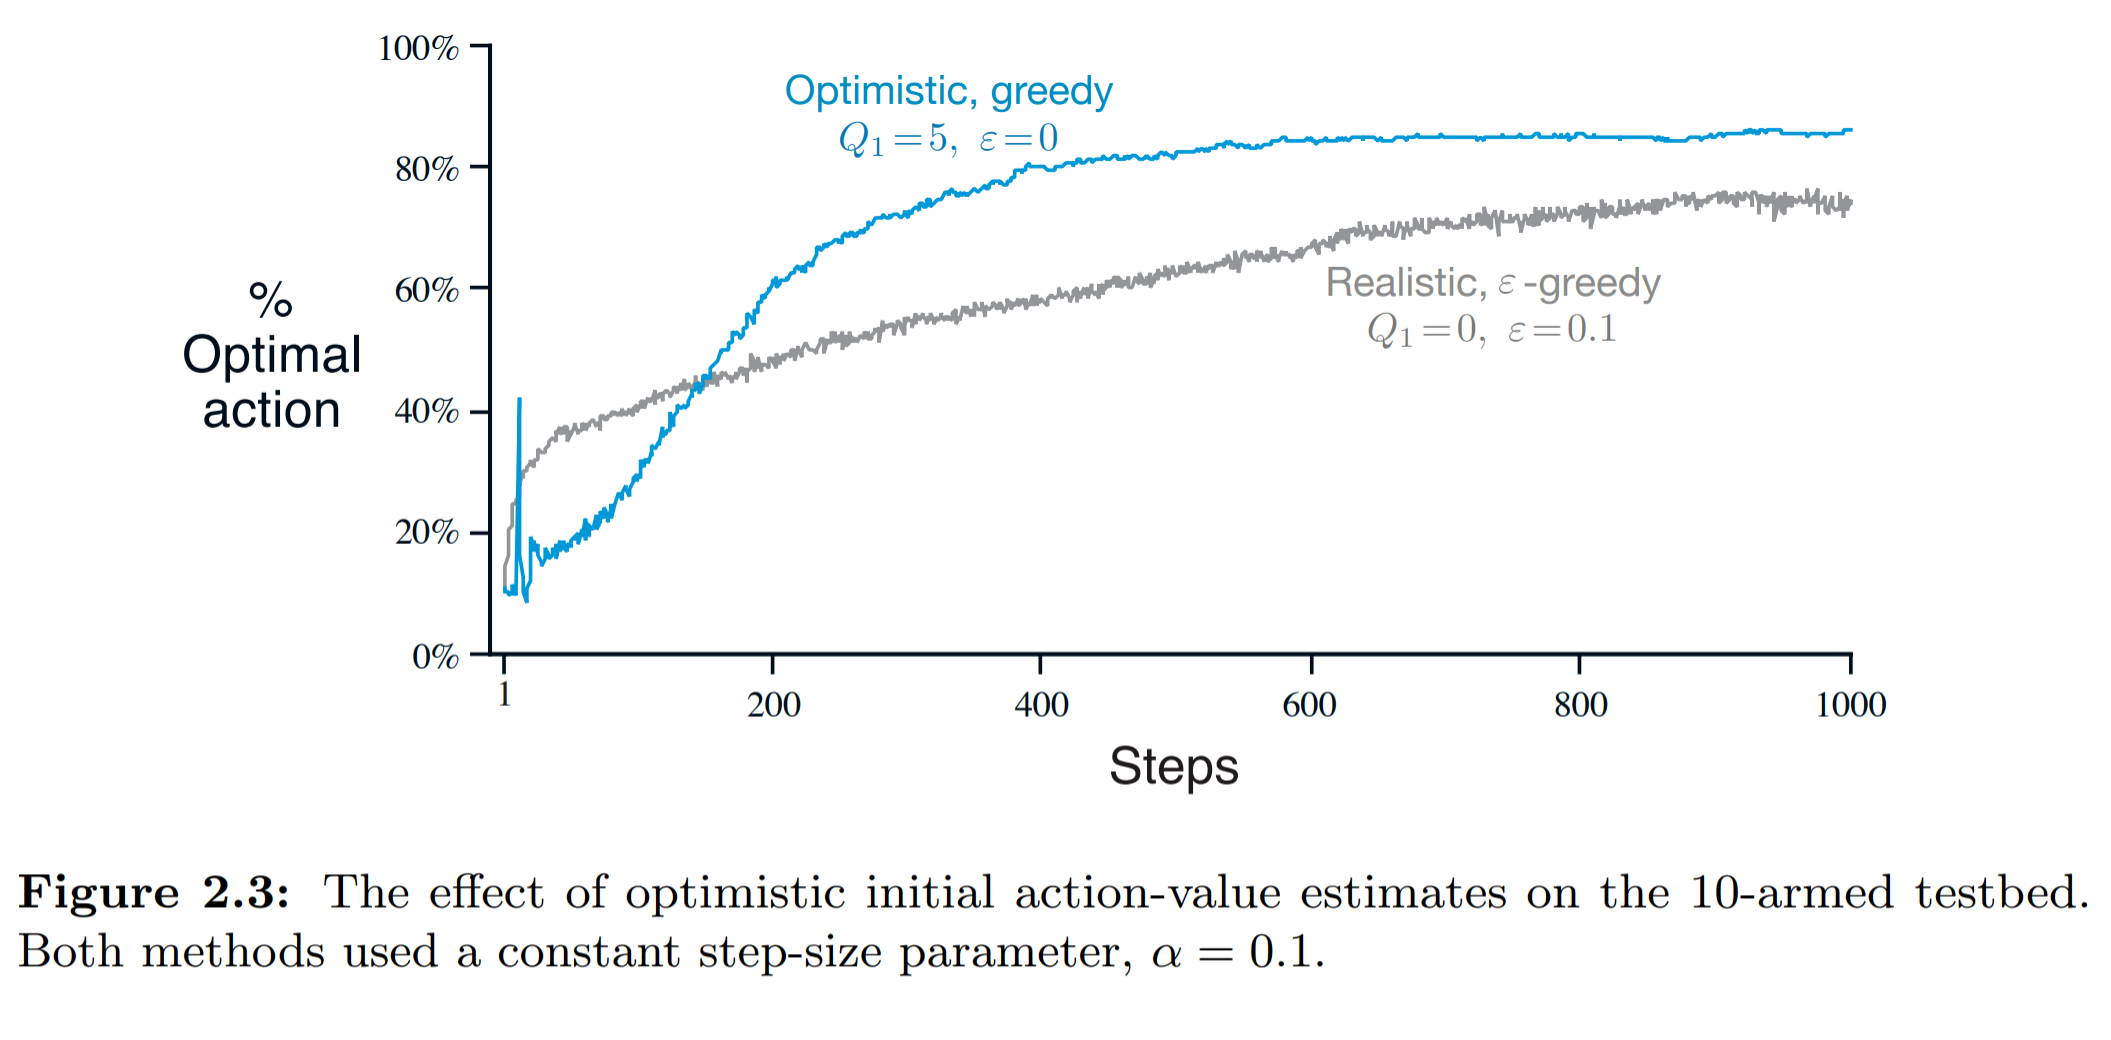
\includegraphics[width=0.9\linewidth]{figures/figure_2dot3.png}
\end{figure}
\smallspace

%Answer: Because the initial values are optimistic, whatever actions are selected on the very first plays will disappoint, and will not be reselected until all the other actions have been tried at least once. Thus, the first 10 plays will just be a sweep through the 10 actions in some random order. The \% optimal action on these 10 plays will thus be at the 10\% chance level. The first opportunity to make a better than chance action selection will be on the 11th play. This is the first spike in the graph. This is where the action that did best in the previous 10 plays is selected again. This action naturally has a greater than chance probability of being the optimal action. However, even if it is optimal, it still disappoints because its action value estimate is still optimistic. Remember, these action-value estimates are computed with a constant step-size parameter and shift only gradually from their initial values to the level of the observed rewards. Thus, although the action on the 11th play was the one that did best on the first 10 plays, on the 11th play its value will be pushed down, closer to its real value rather its optimistic value. On the 12th play the action that did second best in the first 10 plays will be selected, and on the 13th play the action that did third best will be selected. And so on. By trial 21 we can expect a second spike, but it will be less well defined because the values are starting to become more accurate and less optimistic.
